\documentclass[10pt]{article}
\usepackage{amsfonts}
\usepackage{fancyhdr}
\usepackage{comment}
\usepackage[letterpaper, top=2.5cm, bottom=2.5cm, left=2.2cm, right=2.2cm]%
{geometry}
\usepackage{amsmath}
\usepackage{subfig}
\usepackage{mathtools}
\usepackage{changepage}
\usepackage{enumitem}
\usepackage{amssymb}
\usepackage{graphicx}
\usepackage{hyperref}
\usepackage{listings}
\usepackage{color}
\usepackage{textcomp}
\usepackage{courier}

\definecolor{listinggray}{gray}{0.9}
\definecolor{lbcolor}{rgb}{0.96,0.96,0.96}
\lstset{
    backgroundcolor=\color{lbcolor},
    tabsize=4,
    rulecolor=,
    language=Python,
        basicstyle=\footnotesize\ttfamily,
        upquote=true,
        aboveskip={1.0\baselineskip},
        columns=fixed,
        extendedchars=true,
        breaklines=true,
        prebreak = \raisebox{0ex}[0ex][0ex]{\ensuremath{\hookleftarrow}},
        frame=single,
        showtabs=false,
        showspaces=false,
        showstringspaces=false,
        identifierstyle=\ttfamily,
        keywordstyle=\color[rgb]{0,0,1},
        commentstyle=\color[rgb]{0.133,0.545,0.133},
        stringstyle=\color[rgb]{0.627,0.126,0.941},
}

\newcommand{\by}{\mathbf{y}}

\begin{document}

    \title{SDS 383D, Exercises 3: Linear smoothing and Gaussian processes}
    \author{Tyler Buffington}
    \date{\today}
    \maketitle

    \section*{Curve fitting by linear smoothing}
    \begin{enumerate}[label=(\Alph*)]
    \item
    
    We begin with the linear regression equation:
    $$y_i = \beta x_i + \epsilon_i$$
       
    Recall that we derived the least-squares estimator for multiple regression:

    $$\hat{\beta} = (X^TX)^{-1}X^Ty$$

    For the case with the means subtracted, this is equivalent to 
        
    $$\frac{\sum_{i=1}^{n}x_iy_i}{\sum_{i=1}^{n}x_i^2}$$

    Back to our regression equation for one value, but for an new point, $x^*$

    $$\hat{y}^* = \hat{\beta}x^*$$

    Note that the error term is excluded because it has mean zero. Substituting in what we derived for $\hat{\beta}$:
    $$\hat{y^*} =\frac{\sum_{i=1}^{n}x_iy_i}{\sum_{i=1}^{n}x_i^2}x^*$$

    which can then be written like:

    $$\hat{y}^* = \sum_{i=1}^{n}w(x_i,x^*)y_i$$
    where
    $$w(x_i,x^*)= \frac{x_ix^*}{\sum_{j=1}^{n}x_j^2}$$
    This smoothes the data by collapsing it to the least-squares regression line. The K-nearest-neighbor smoothing will conversely take the average of the K nearest points (by x). It is worth noting that in the linear smoother, data points with x values very far away from $\bar{x}$ are assigned large weights.	

    \item
    The code for the analysis can be found in kernel\_smooth.py. The resulting plot is shown below: 
    \begin{figure}[htb] \centering
    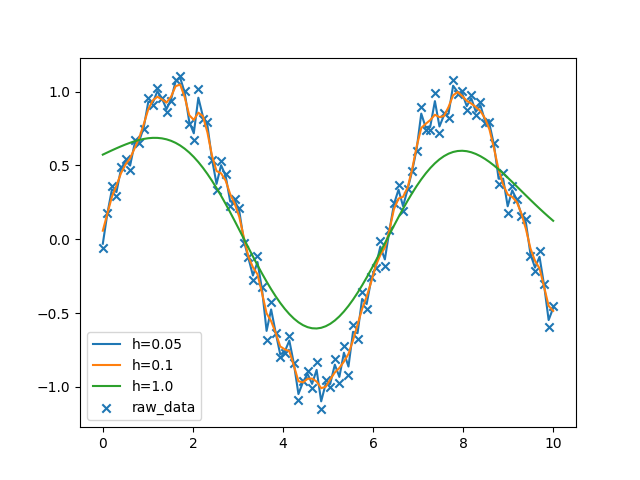
\includegraphics[width=0.95\textwidth]{./gaussian_kernel.png}
    \caption{The fit for different bandwidth values.}
    \label{fig:gaussian_kernel}
    \end{figure}
    
    This plot illustrates the bias-variance tradeoff: as h increases, the fit becomes less noisy, but more biased. In the limit as h goes to $\inf$, the fit becomes a flat line at the mean because this would mean that all points have equal weight. On the other hand, as h goes to zero, the fit would match the data exactly, which is also not useful because it would pick up the noise from the raw data as well.
	\end{enumerate}

    \section*{Cross validation}
    \begin{enumerate}[label=(\Alph*)]
    \item
    See cross\_validaiton.py.
    \item
    The methodology is detailed in bandwidth\_select.py. The smooth function was chosen to be $y=x^3$ and tthe wiggly function was chosen to be $y=sin(50x)$. The error as a function of bandwidth, h, is plotted below:

    \begin{figure}[htb] \centering
    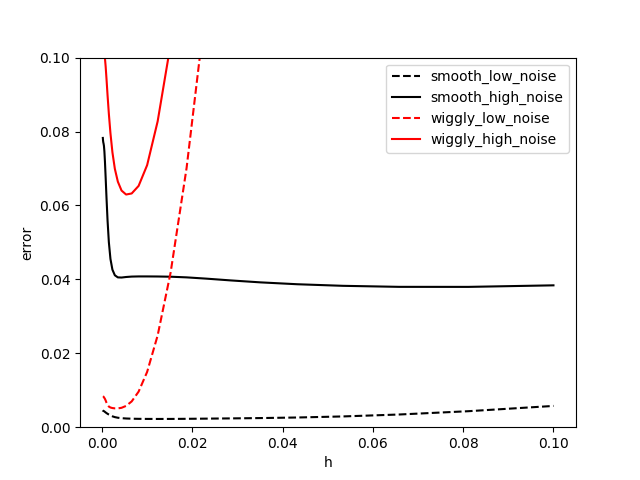
\includegraphics[width=0.95\textwidth]{./h_select.png}
    \caption{the error for different bandwidth values.}
    \label{fig:h_select}
    \end{figure}

    the main features are that the noisy functions have higher errors at the optimal h, and the noise also increases the value for the optimal h. the optimal fits are shown for the four cases below in Figure \ref{results}

    \begin{figure}[!b]
    \begin{center}
    %
    \subfloat[smooth low noise]{%
      \label{fig:sl} 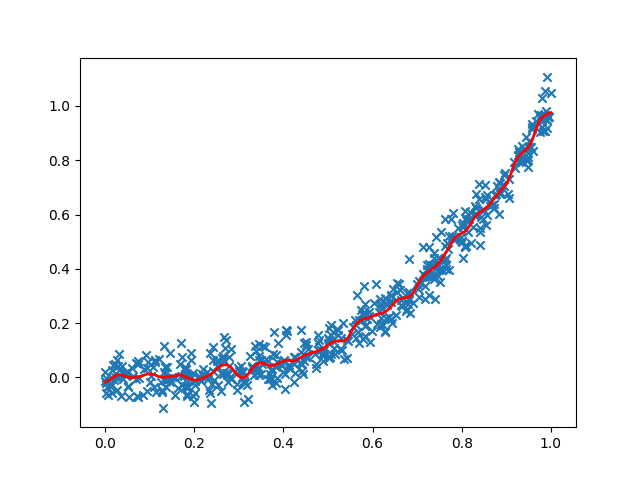
\includegraphics[width=7cm,keepaspectratio]{./smooth_low_noise.png}
    }%
    \subfloat[smooth high noise]{%
     \label{fig:sh} 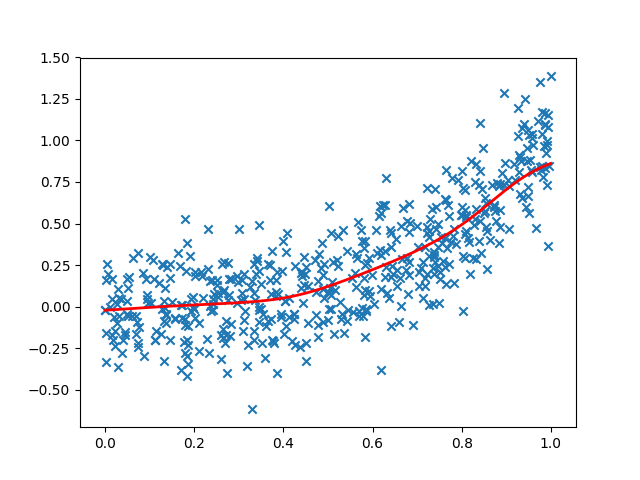
\includegraphics[width=7cm,keepaspectratio]{./smooth_high_noise.png}
    }\\ %  ------- end of the first row ----------------------%
    \subfloat[wiggly low noise]{%
      \label{fig:wl} 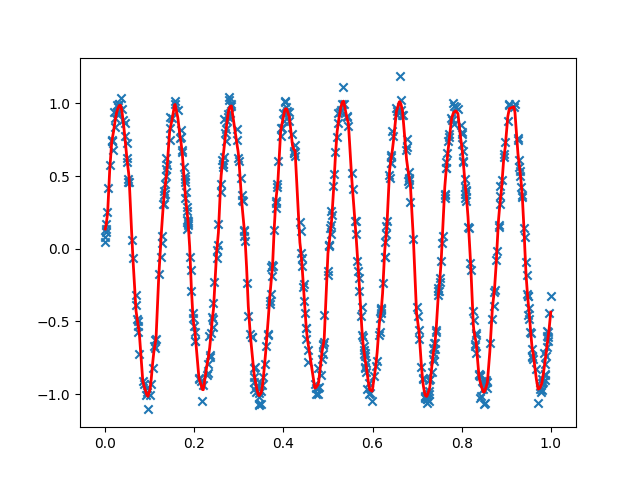
\includegraphics[width=7cm,keepaspectratio]{./wiggly_low_noise.png}
    }%
    \subfloat[wiggly high noise]{%
     \label{fig:wh} 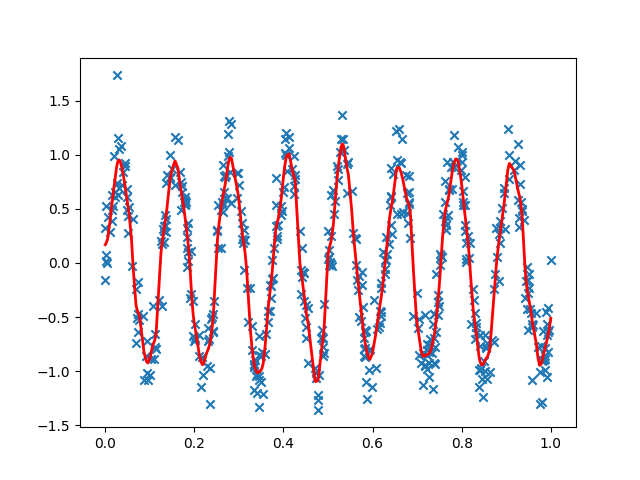
\includegraphics[width=7cm,keepaspectratio]{./wiggly_high_noise.png}
    }\\ %  ------- end of the second row ----------------------%

    \end{center}
    \caption{The fits at the optimal h for the four cases.}
    \label{fig:results}
    \end{figure}
    \clearpage
    \end{enumerate}
    \section*{Local polynomial regression}
        \begin{enumerate}[label=(\Alph*)]
        \item

        For points u in a neighborhood of the target point x, define the polynomial
        $$g_x(u;a) = a_0 + \sum_{k=1}^Da_k(u-x)^k$$
        where 
        $$\hat{a} = \arg \min_{R^{D+1}}  \sum_{i=1}^{n}w_i\{y_i-g_x(x_i;a)\}^2$$
        substitute in $g_x(x_i;a)$

        $$\hat{a} = \arg \min_{R^{D+1}}  \sum_{i=1}^{n}w_i\{y_i-a_0 - \sum_{k=1}^Da_k(x_i-x)^k\}^2$$
        Then define matrix R such that $R_{i,j} = (x_i-x)^{j-1}$, so then we get 

        $$\hat{a} = \arg \min_{R^{D+1}}  \sum_{i=1}^{n}w_i\{y_i-Ra\}^2$$
        If we define W to be a diagonal matrix where $W_{i,i}=w_i$, and all off diagonal terms are zero, we get

        $$\hat{a} = \arg \min_{R^{D+1}}  \{y-Ra\}^TW\{y-Ra\}$$
        Then evaluate derivative and set equal to zero to minimize:

        $$\frac{d}{da}\{y-Ra\}^TW\{y-Ra\}$$
        $$=\frac{d}{da}[y^TWy-2y^TWRa+a^TR^TWRa]$$
        $$=-2R^TWy+2R^TWRa = 0$$
        $$R^TWRa=R^TWy$$
        $$a = (R^TWR)^{-1}R^TWy$$
        We can then define a matrix $M=(R^TWR)^{-1}W$ so that we get the final clean form:
        $$a=My$$
        \item
        Beginning with result from part A:
        $$a = (R^TWR)^{-1}R^TWy$$


        $$=\Bigg(
        \begin{bmatrix}
        1 & \dots & 1 \\ 
        (x_1-x) & \dots & (x_n-x)
        \end{bmatrix}
        \begin{bmatrix} 
        w_1 & \dots & 0 \\ 
        \vdots & \ddots & \vdots \\ 
        0 & \dots & w_n 
        \end{bmatrix}
        \begin{bmatrix}1&(x_1-x)\\ 
        \vdots & \vdots \\ 
        1 & (x_n - x) \end{bmatrix}
        \Bigg)^{-1}
        \begin{bmatrix} 
        w_1 & \dots & 0 \\ 
        \vdots & \ddots & \vdots \\ 
        0 & \dots & w_n 
        \end{bmatrix}
        \begin{bmatrix} 
        1 &(x_1-x) \\ 
        \vdots & \vdots \\ 
        1 & (x_n - x) \end{bmatrix}
        \begin{bmatrix}
        y_1\\
        \vdots\\
        y_n
        \end{bmatrix}
        $$

        $$=\begin{bmatrix}
        \sum_{i=1}^nw_i & \sum_{i=1}^{n}w_i(xi-x) \\
        \sum_{i=1}^{n}w_i(x_i-x) & \sum_{i=1}^nw_i(x_i-x)^2
        \end{bmatrix}^{-1}
        \begin{bmatrix}
        \sum_{i=1}^{n}y_iw_i \\
        \sum_{i=1}^n y_iw_i(x_i-x)
        \end{bmatrix}$$

        $$=\frac{1}{\sum_{i=1}^nw_i \sum_{i=1}^nw_i(x_i-x)^2 - (\sum_{i=1}^nw_i (x_i-x))^2}
        \begin{bmatrix}
        \sum_{i=1}^nw_i(x_i-x)^2 & -\sum_{i=1}^{n}w_i(x_i-x) \\
        -\sum_{i=1}^{n}w_i(x_i-x) & \sum_{i=1}^nw_i     
        \end{bmatrix}
        \begin{bmatrix}
        \sum_{i=1}^{n}y_iw_i \\
        \sum_{i=1}^n y_iw_i(x_i-x)
        \end{bmatrix}$$

        $$=\frac{1}{\sum_{i=1}^nw_i \sum_{i=1}^nw_i(x_i-x)^2 - (\sum_{i=1}^nw_i (x_i-x))^2}
        \begin{bmatrix}
        \sum_{i=1}^nw_i(x_i-x)^2\sum_{i=1}^ny_iw_i - \sum_{i=1}^nw_i(x_i-x)\sum_{i=1}^ny_iw_i(x_i-x) \\
        -\sum_{i=1}^nw_i(x_i-x)\sum_{i=1}^ny_iw_i+\sum_{i=1}^nw_i\sum_{i=1}^ny_iw_i(x_i-x)
        \end{bmatrix}$$

        It can be seen that at the target point x, $\hat{f} = a_0$, so we get 
        $$\hat{f} =  \frac{\sum_{i=1}^nw_i(x_i-x)^2\sum_{i=1}^ny_iw_i - \sum_{i=1}^nw_i(x_i-x)\sum_{i=1}^ny_iw_i(x_i-x)}{\sum_{i=1}^nw_i \sum_{i=1}^nw_i(x_i-x)^2 - (\sum_{i=1}^nw_i (x_i-x))^2}$$

        Let $s_1 = \sum_{i=1}^nw_i(x_i-x)$ and $s_2 = \sum_{i=1}^nw_i(x_i-x)^2$. So then we get:

        $$\hat{f} = \frac{s_2\sum_{i=1}^ny_iw_i-s_1\sum_{i=1}^ny_iw_i(x_i-x)}{\sum_{i=1}^nw_is_2 - s_1\sum_{i=1}^nw_i(x_i-x)}$$

        $$= \frac{\sum_{i=1}^ny_iw_i\big(s_2-s_1(x_i-x)\big)}{\sum_{i=1}^nw_i\big(s_2-s_1(x_i-x)\big)}$$

        Define $w_i^* = w_i\big(s_2 - s_1(x_i-x)\big)$, so then we get the desired form:
        $$\hat{f} = \frac{\sum_{i=1}^nw_i^*y_i}{\sum_{i=1}^nw_i^*}$$

    \end{enumerate}
\end{document}
\grid
